\documentclass[11pt]{article}
\newcommand{\oa}{\overline{a}}
\newcommand{\ob}{\overline{b}}
\newcommand{\oc}{\overline{c}}
\newcommand{\oi}{\overline{i}}

\newcommand{\integermodn}[1][n]{\Z/#1\Z}
\newcommand{\integermodnmul}[1][n]{(\Z/#1\Z)^{\times}}
\newcommand{\order}[1]{\left|#1\right|}
\newcommand{\modb}[1]{\left(mod \;\; #1 \right)}
\newcommand{\aut}[1]{Aut\left(#1\right)}
\newcommand{\actson}{\ensuremath{\curvearrowright}}

\newcommand{\heading}[1]{(#1)}
\newcommand{\bheading}[1]{\textbf{(#1)}}

% arg1=pdfurl arg2=pagenum arg3=text
\usepackage{url}
\usepackage{hyperref}
\hypersetup{colorlinks=true, linktoc=all, linkcolor=blue}
\newcommand{\linkbook}[3][../../abstract_algebra_dummit_and_foote.pdf]{
    \noindent\href[page=#2]{#1}{\urlstyle{rm}{#3}}
}

\usepackage[a4paper, total={6in, 8in}, margin=0.5in]{geometry}

\usepackage{listings}
\usepackage{hyperref}
\graphicspath{{assets/}}



\begin{document}

\section*{Problem 1}
\begin{enumerate}
    \item Show 
    \[
        \forw^s z(x) = \sum_{i=0}^s (-1)^{s-i} \binom{s}{i} z(x+ih)
    \]
    \begin{proof}
        If $s=1$, $\forw z(x) = -z(x) + z(x+h) = \sum_{i=0}^s (-1)^{s-i} \binom{s}{i} z(x+ih)$. If $s>1$, assume
        \[
            \forw^{s-1} z(x) = \sum_{i=0}^{s-1} (-1)^{s-1-i} \binom{s-1}{i} z(x+ih)
        \]
        Therefore,
        \begin{align*}
            \forw^s z(x)
                &= \forw \p{\forw^{s-1} z(x)} \\
                &= \forw \p{
                    \sum_{i=0}^{s-1} \p{(-1)^{s-1-i} \binom{s-1}{i} z(x+ih)}
                } \\ 
                &= \sum_{i=0}^{s-1} \p{(-1)^{s-1-i} \binom{s-1}{i} z(x+(i+1)h)}
                    - \sum_{i=0}^{s-1} \p{(-1)^{s-1-i} \binom{s-1}{i} z(x+ih)} \\
                &= \pb{
                    \sum_{j=1}^{s-1} \p{(-1)^{s-j} \binom{s-1}{j-1} z(x+jh)} + (-1)^{s-s} \binom{s-1}{s-1} z(x+sh)
                } \\ 
                &\quad\quad - (-1) \pb{
                    \sum_{j=1}^{s-1} \p{(-1)^{s-j} \binom{s-1}{j} z(x+jh)} - (-1)^{s} z(x)
                } \\
                &= \sum_{j=1}^{s-1} \p{(-1)^{s-j} \pb{ \binom{s-1}{j-1} + \binom{s-1}{j} } z(x+jh)}
                + z(x+sh)
                + (-1)^s z(x) \\
                &= \sum_{i=0}^s (-1)^{s-i} \binom{s}{i} z(x+ih)
        \end{align*}
        where last step is given by the recurrence relation 
        \[
            \binom{s}{j} = \binom{s-1}{j-1} + \binom{s-1}{j}
        \]
    \end{proof}
    \item Show 
    \[
        \sum_{i=0}^s (-1)^{s-i} \binom{s}{i} i^j = 0    
    \]
    \item Give a rigorous, shorter proof of $\forw^s z(x) = \sO(h^s)$
    \begin{proof}
        Given $z(x)$ has $s$ continuous derivatives, use mean value theorem repeatedly. We claim that 
        \[
            \forw^s z(x) = h^s z^{(s)} (\eta^{(s)})
            \quad \quad \text{for some} \quad \quad 
            \eta^{(s)} \in (x, x + sh)
        \]
        Use induction. When $s=1$, 
        \[
             \forw z(x) = h \frac{z(x+h) - z(x)}{h} = h z^{(1)}(\eta^{(1)})
             \quad \quad \eta^{(1)} \in (x, x+h)
        \]
        when $s>1$ assume $\forw^{s-1} z(x) = h^{s-1} z^{(s-1)} (\eta^{(s-1)})$ for some $\eta^{(s-1)} \in (x, x + (s-1)h)$, then 
        \[
            \forw^s z(x) 
                = \forw (\forw^{s-1} z(x)) 
                = h^s \frac{
                    z^{(s-1)}(\eta^{(s-1)} + h) - z^{(s-1)}(\eta^{(s-1)})
                }{h}
                = h^s z^{(s)} (\eta^{(s)})
        \]
        for some $\eta^{(s)} \in (x, x + sh)$. 
    \end{proof}
\end{enumerate}


\section*{Problem 2 (textbook 166 8.1)}
Prove 
\[
    \back + \forw = 2\avg\cent 
    \quad \quad \text{and} \quad \quad
    \back\forw = \cent^2    
\]
\begin{proof}
    Note $\back = \id - \shift^{-1}$, $\forw = \shift - \id$, $\cent = \shift^{1/2} - \shift^{-1/2}$, and $\avg = 1/2(\shift^{1/2} + \shift^{-1/2})$. So 
    \begin{align*}
        \back+\forw 
            &= \id - \shift^{-1} + \shift - \id \\
            &= \shift - \shift^{-1} \\
            &= (\shift^{1/2} + \shift^{-1/2})(\shift^{1/2} - \shift^{-1/2}) \\
            &= 2 \avg\cent
    \end{align*}
    and
    \begin{align*}
        \back\forw
            &= (\id - \shift^{-1})(\shift - \id) \\
            &= \shift - \id - \id + \shift^{-1} \\
            &= (\shift^{1/2} - \shift^{-1/2})^2 \\
            &= \cent^2
    \end{align*}
\end{proof}


\section*{Problem 3 (textbook 167 8.5)}
Consider finite difference approximations to the derivative that use one point to the left and $s\geq 1$ points to the right of $x$
\begin{enumerate}
    \item Determine constants $\alpha_j$, $j=1,2,\cdots$ such that
    \[  
        \diff = \frac{1}{h} \p{
            \beta \back + \sum_{j=1}^{\infty} \alpha_j \forw^j
        }
    \]
    where $\beta \in\R$ is given.
    \begin{proof}
        Write the formula w.r.t. $\forw$ and use the following expansion to determine $\alpha_j$s
        \[
            \forw = \shift - \id = \id - e^{-h\diff}
            = \id - \sum_{i=0}^{\infty} \frac{(-h\diff)^i}{i!}
            = \sum_{i=1}^{\infty} \frac{(-h\diff)^i}{i!}
        \]
        Express $\back$ as an expansion of $\forw$
        \[
            \back 
            = \id - \shift^{-1}
            = \id - \p{\id + \forw}^{-1}
            = \id - \sum_{i=0}^{\infty} (-1)^{i} \forw^i
            = \sum_{i=1}^{\infty} (-1)^{i+1} \forw^i
        \]
        Now we have 
        \begin{align*}
            h\diff 
                &= \beta \back + \sum_{j=1}^{\infty} \alpha_j \forw^j \\
                &= \sum_{j=1}^{\infty} \p{\beta(-1)^{j+1} + \alpha_j} \forw^j \
        \end{align*}
        But note
        \[
            h\diff 
            = \ln (\shift) 
            = \ln (\id + \forw)
            = \sum_{j=1}^{\infty} \frac{(-1)^{j+1}}{j} \forw^j
        \]
        Therefore,
        \[
            \frac{(-1)^{j+1}}{j} = \beta(-1)^{j+1} + \alpha_j
            \quad \quad \Rightarrow \quad \quad
            \alpha_j = (-1)^{j-1} (\frac{1}{j} - \beta)
        \]
    \end{proof}
    \item Given integer $s\geq 1$, show how to choose parameter $\beta$ so that 
    \[
        \diff = \frac{1}{h} \p{
            \beta \back + \sum_{j=1}^{s} \alpha_j \forw^j
        } + \sO(h^{s+1})
        \quad \quad h\to 0
    \]
    \begin{proof}
        From conclusion of previous, we can write 
        \begin{align*}
            \diff 
                &= \frac{1}{h} \p{
                    \beta \back + \sum_{j=1}^{\infty} \alpha_j \forw^j
                } \\
                &= \frac{1}{h} \p{
                    \beta \back + \sum_{j=1}^{s} \alpha_j \forw^j
                }
                + \frac{1}{h}\alpha_{s+1} \forw^{s+1}
                + \frac{1}{h}\sum_{j=s+2}^{\infty} \alpha_j \forw^j \\ 
                &= \frac{1}{h} \p{
                    \beta \back + \sum_{j=1}^{s} \alpha_j \forw^j
                }
                + \frac{1}{h}\alpha_{s+1} \forw^{s+1}
                + \sO(h^{s+1}) \tag{from Q1 $\forw^s = \sO(h^s)$} \\
                &= \frac{1}{h} \p{
                    \beta \back + \sum_{j=1}^{s} \alpha_j \forw^j
                }
                + \sO(h^{s+1})
        \end{align*}
        where last equality holds if and only if $\alpha_{s+1} = 0$, from previous, we have 
        \[
            \alpha_{s+1} = (-1)^{s} (\frac{1}{s+1} - \beta)
            \quad \quad \Rightarrow \quad \quad
            \beta = \frac{1}{s+1}
        \]
    \end{proof}
\end{enumerate}


\section*{Problem 4}
Implementation of 5-point centered difference approximation to the poisson equation $\nabla^2 u = f$ on $\Omega = (0,1)\times (0,1)$ with Dirichlet boundary condition is in \hyperref[q4code]{appendix}. The maximum error is given as follows
\begin{center}
    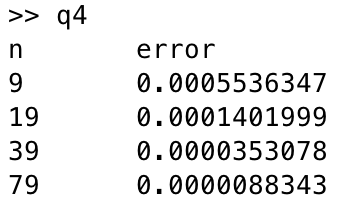
\includegraphics[width=1.5in]{p4output}
\end{center}
The rate of convergence for five point method is $\Dx^2$. The result agrees with the theory, i.e. approximately, as $n$ doubles, $\Dx=\Dy$ halfs, and error decreases by a factor of 4.


\section*{Problem 5}
Implementation of 5-point centered difference approximation to possion equation $\nabla^2 u = f$ on $\Omega = (0,1)^2$ with Dirichlet boundary conditions on three sides and a Neumann boundary condition on the fourth side is in \hyperref[q5code]{appendix}. For both approximation method to the Neumann boundary condition, we simply change how we construct $A$ and $b$ matrix while leaving the rest the same. 
\begin{enumerate}
    \item \bheading{first order} Approximate $u_x(1,y)$ by $\textstyle\frac{1}{\Dx} \varDelta_{-,x}$, we have the following boundary condition
    \begin{equation}\label{eq1}
        \frac{u_{n+1,j} - u_{n,j}}{\Dx} = -\frac{1}{4}
        \quad \quad \Rightarrow \quad \quad
        u_{n+1,j} = -\frac{1}{4} \Dx + u_{n,j}
    \end{equation}
    The discretization of $\textstyle\frac{\partial^2}{\partial x^2}$ as $\varDelta_{0,x}$ at the Neumann boundary, i.e. $(n\Dx, j\Dy)$ for $j=1,2,\cdots,n$, is
    \begin{align*}
        \frac{u_{n+1,j} - 2u_{n,j} + u_{n-1,j}}{\Dx^2}
            &= \frac{\p{-\frac{1}{4} \Dx + u_{n,j}} - 2u_{n,j} + u_{n-1,j}}{\Dx^2} \\
            &= -\frac{1}{4\Dx} + \frac{-u_{n,j} + u_{n-1,j}}{\Dx^2}
    \end{align*}
    we change the corresponding entries in $A$ and $b$ to reflect this.
    \[
        A_{nj,nj} = -\frac{1}{\Dx^2} - \frac{2}{\Dy^2}
        \quad \quad
        b_{nj} \text{ += } \frac{1}{4\Dx}
    \]
    \item \bheading{second order} Approximate $u_x(1,y)$ by $\textstyle\frac{1}{\Dx} (\varDelta_{-,x} + \frac{1}{2} \varDelta^2_{-,x})$, we have the following boundary condition at $j=1,2,\cdots, n$
    \begin{equation} \label{eq2}
        \frac{\frac{3}{2} u_{n+1,j} - 2u_{n,j} + \frac{1}{2}u_{n-1,j}}{\Dx} = -\frac{1}{4}
        \quad \quad \Rightarrow \quad \quad
        u_{n+1,j} = -\frac{1}{6} \Dx + \frac{4}{3} u_{n,j} - \frac{1}{3} u_{n-1,j}
    \end{equation}
    The discretization of $\textstyle\frac{\partial^2}{\partial x^2}$ as $\varDelta_{0,x}$ at the Neumann boundary is
    \begin{align*}
        \frac{u_{n+1,j} - 2u_{n,j} + u_{n-1,j}}{\Dx^2}
            &= \frac{\p{
                -\frac{1}{6} \Dx + \frac{4}{3} u_{n,j} - \frac{1}{3} u_{n-1,j}
            } - 2u_{n,j} + u_{n-1,j}}{\Dx^2} \\
            &= -\frac{1}{6\Dx} + \frac{-\frac{2}{3} u_{n,j} + \frac{2}{3}u_{n-1,j}}{\Dx^2}
    \end{align*}
    we change the corresponding entries in $A$ and $b$ to reflect this
    \[
        A_{nj, nj} = -\frac{2}{3\Dx^2} - \frac{2}{\Dy^2}    
        \quad \quad
        A_{(n-1)j, nj} = \frac{2}{3\Dx^2}
        \quad \quad
        b_{nj} \text{ += } \frac{1}{6\Dx}
    \]
\end{enumerate}
Note for $i=n+1$, we obtain $\tilde{u}_{n+1,j}$ by evaluating $\textstyle u(1, y) = \frac{1}{2} + \frac{1}{y+1}$ and we obtain $u_{n+1,j}$ by computing \bheading{\ref{eq1}} for 1st order approximation method and \bheading{\ref{eq2}} for 2nd order approximation method. The maximum error is given as follows
\begin{center}
    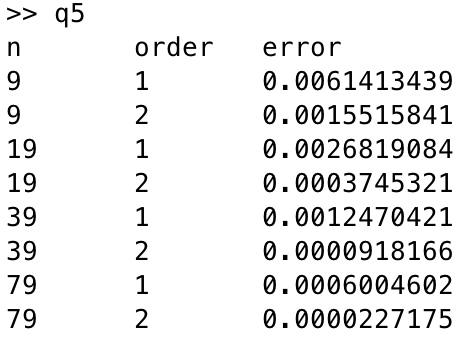
\includegraphics[width=2in]{q5output}
\end{center}
Approximately, as $n$ doubles, $\Dx=\Dy$ halves, error for first order method decreases by a factor of 2 while error for second order method decreases by a factor of 4. The error for first order method appears to be first-order accurate and that for second order method appears to be second-order accurate. Note since we are taking into account the $i=n+1$, the dominant factor in determining rate of convergence is at the Neumann boundary by observation. The rate of convergence of first/second order approximation at boundary agrees with observation.
\begin{figure}[ht]
    \begin{center}
        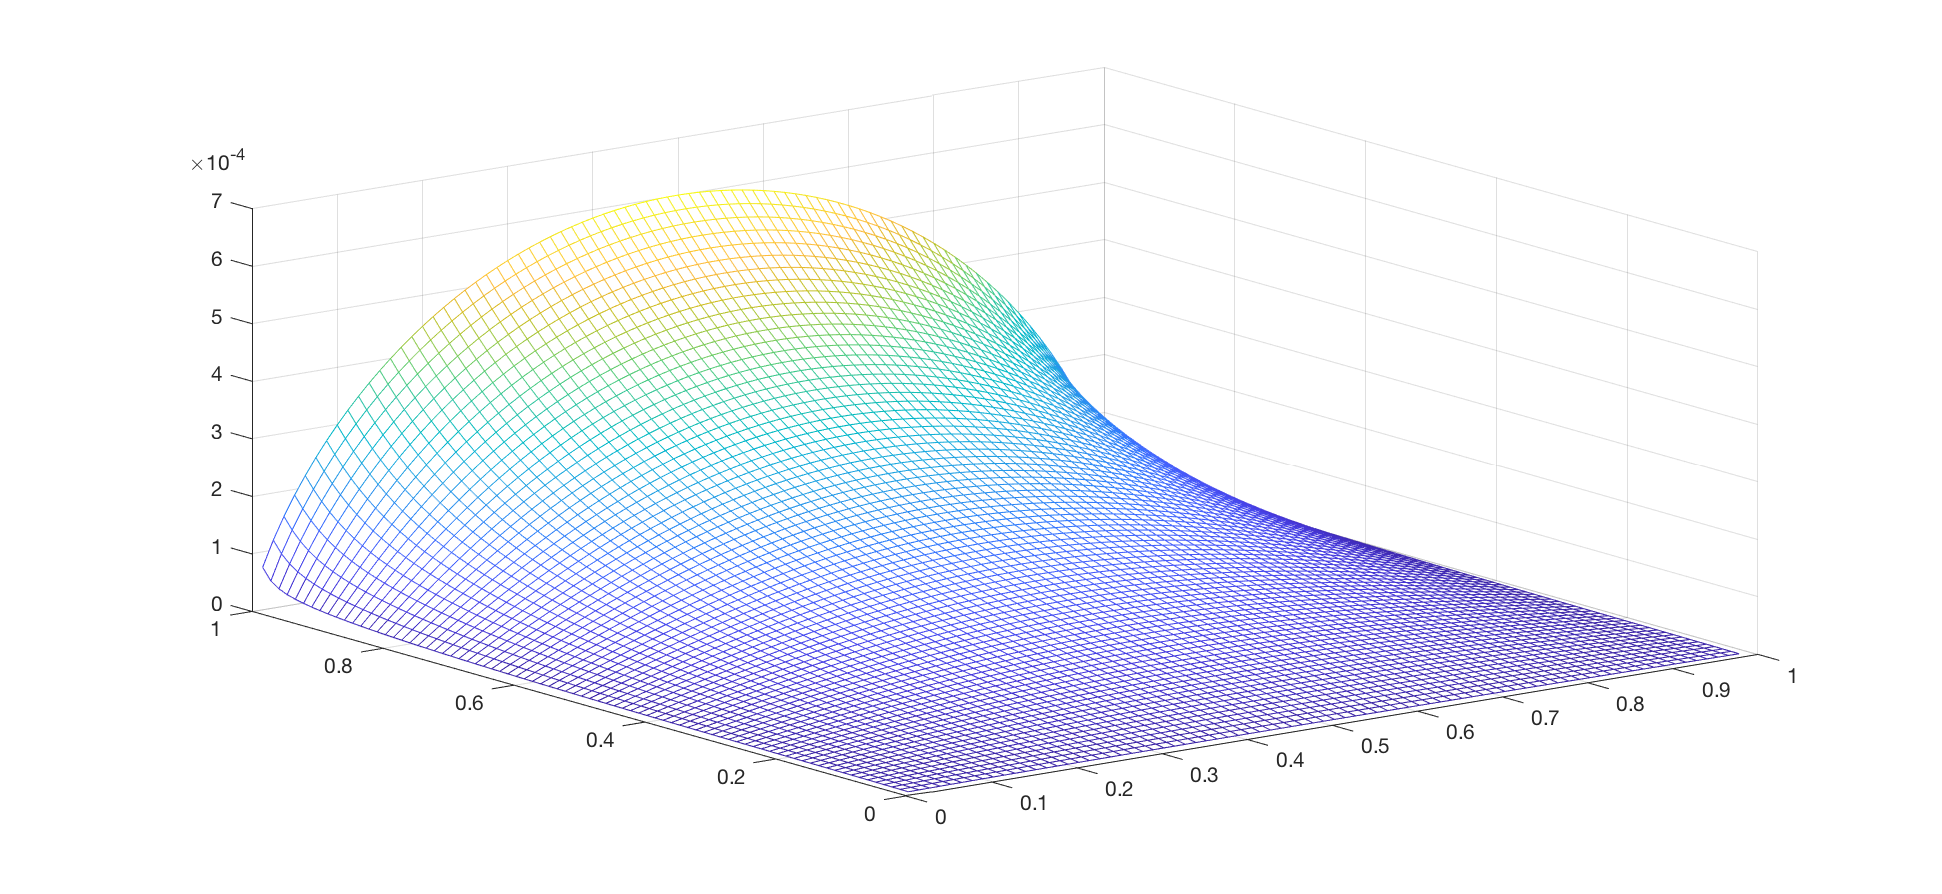
\includegraphics[width=3in]{q5_od_1} 
        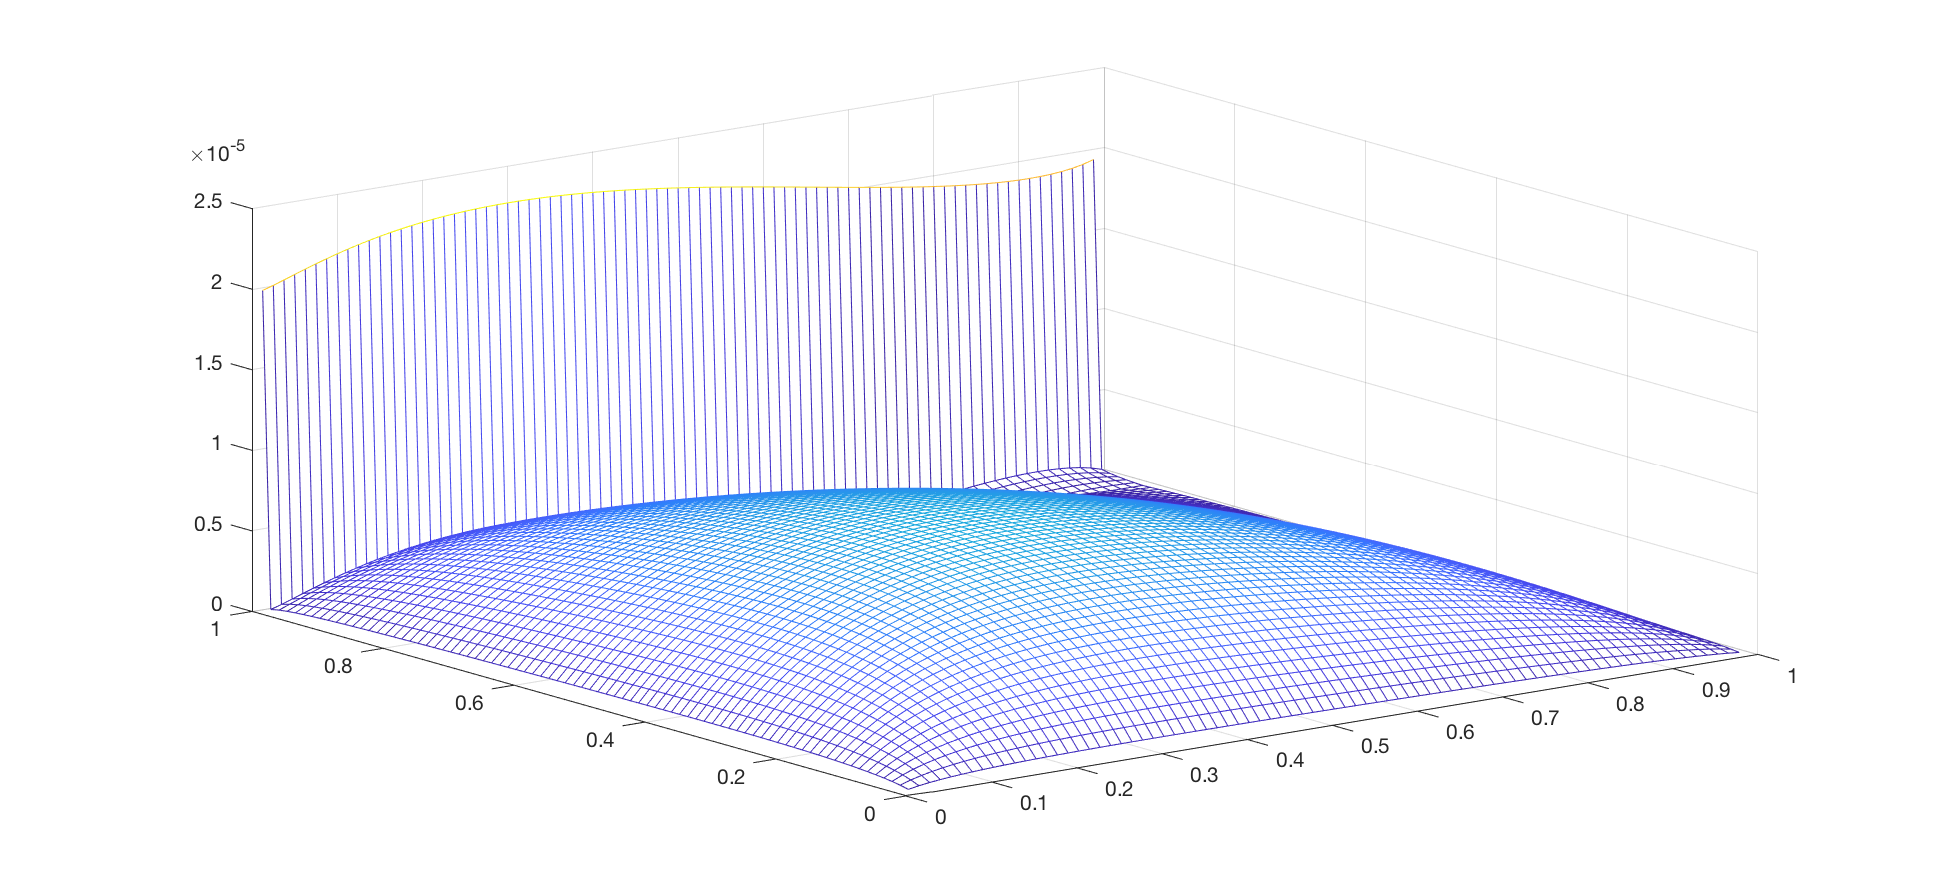
\includegraphics[width=3in]{q5_od_2}
        \caption{error graph for (left) first-order and (right) second-order method (n=79)}
    \end{center}
\end{figure}



\subsection*{Problem 6}
Implementation of 5-point centered difference approximation to possion equation $\nabla^2 u = f$ on $\Omega = \pc{(x,y)\mid x^2+y^2<1}$ with Dirichlet boundary conditions with specified $f$ and $u$ is in \hyperref[q6code]{appendix}. The maximum error is given as follows
\begin{center}
    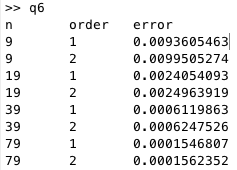
\includegraphics[width=2in]{q6output}
\end{center}
Approximately, as $n$ doubles, $\Dx=\Dy$ halves, and error for both first order and second order method decreases by a factor of 4. The error for both first and second order method at boundary appears to be second-order accurate. This is counterintuitive. However, after plotting the error graph, it seems that error value is dominated by internal grid point estimates. Even though error is decreasing linearly at boundary for first order method, the error at boundary is masked by large error incurred at internal grid points. 
\begin{figure}[ht]
    \begin{center} 
        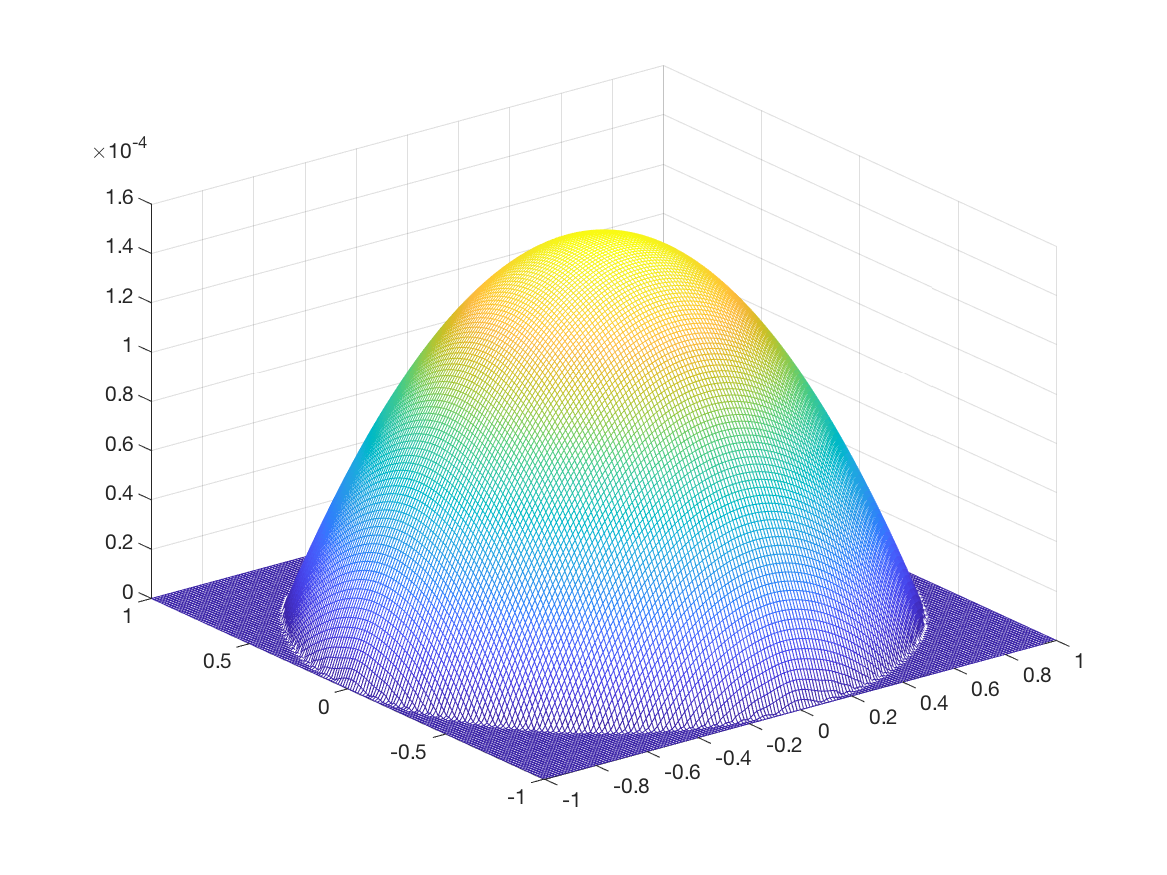
\includegraphics[width=3in]{q6_od_1} 
        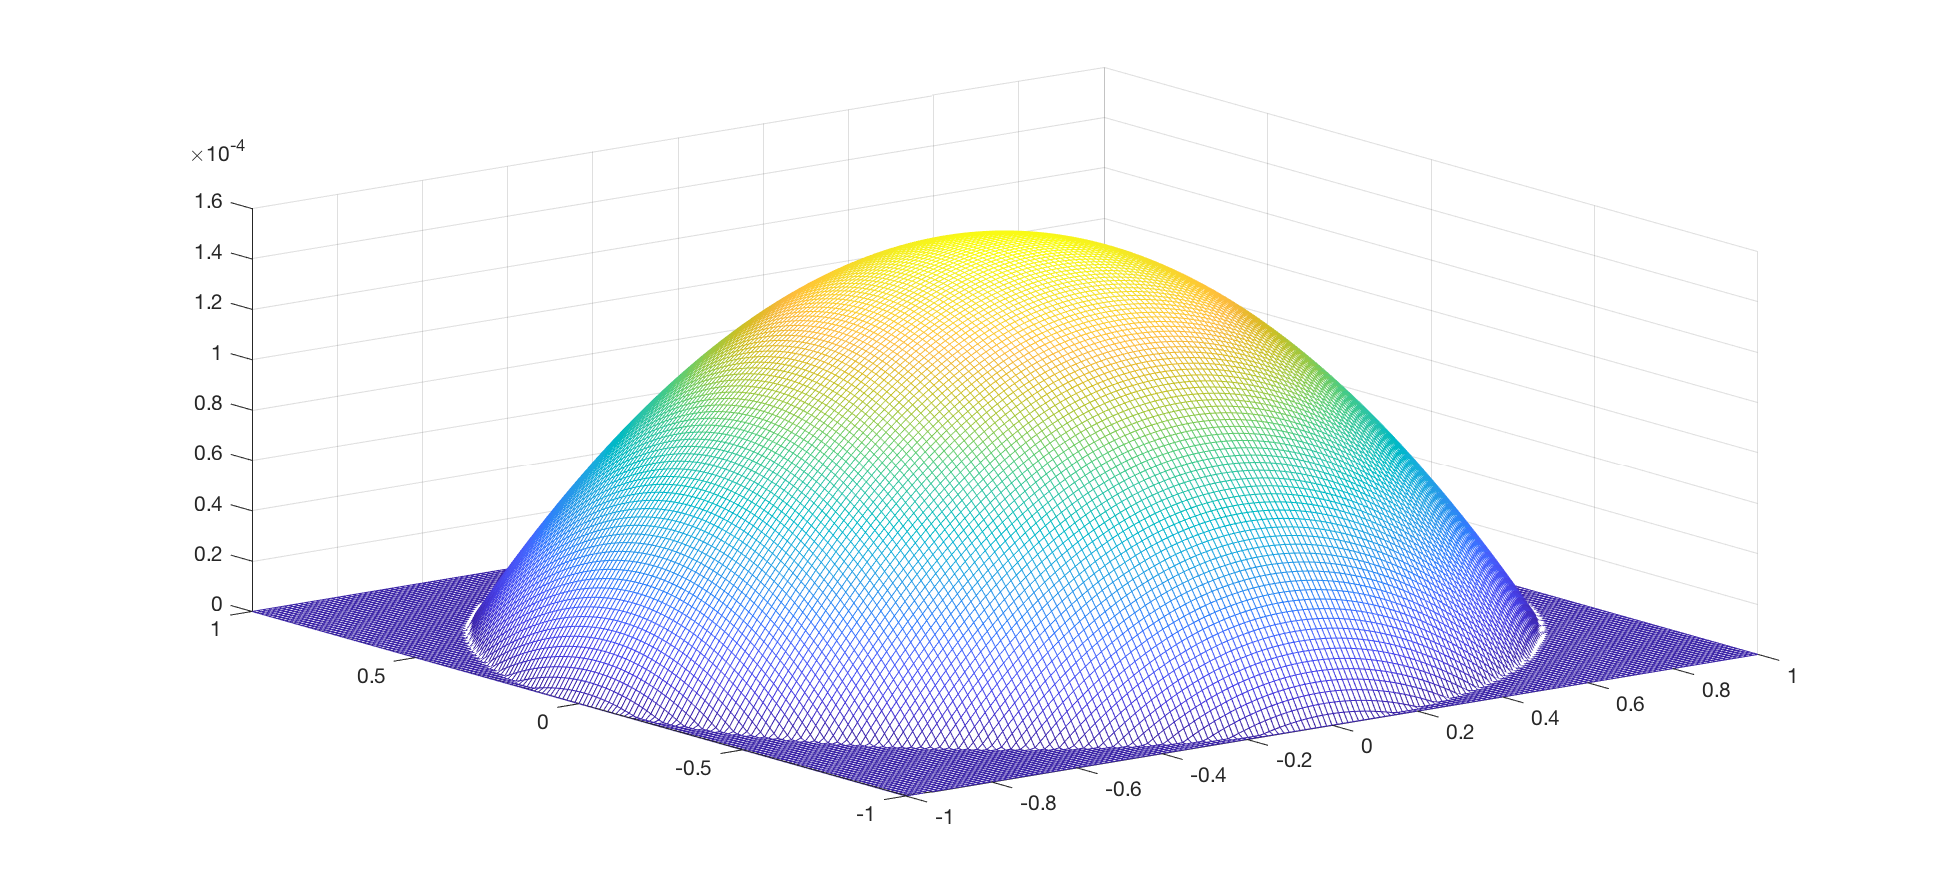
\includegraphics[width=3in]{q6_od_2}
        \caption{error graph for (left) first-order and (right) second-order method (n=79)}
    \end{center}
\end{figure}

\subsection*{Problem 7}

\textit{Upper and Lower Bounds for Inverse Elements of Finite and Infinite Tridiagonal Matrices} \\
\bheading{https://core.ac.uk/download/pdf/82217635.pdf} seems to solve this particular problem

\subsection*{Problem 8}
\textit{BLOCK DIAGONAL DOMINANCE OF MATRICES REVISITED: BOUNDS FOR THE NORMS OF INVERSES AND EIGENVALUE INCLUSION SETS∗}
\bheading{https://arxiv.org/pdf/1712.05662.pdf} seems to solve this particular problem

\subsection*{Problem 9}
\bheading{https://mathoverflow.net/questions/72832/overlapping-gershgorin-disks} seems to solve the problem

\newpage

\section*{Appendix}

\section*{problem 4 code}
\label{q4code}
\lstinputlisting[language=matlab]{code/q4.m}

\newpage
\section*{problem 5 code}
\label{q5code}
\lstinputlisting[language=matlab]{code/q5.m}

\newpage
\section*{problem 6 code}
\label{q6code}
\lstinputlisting[language=matlab]{code/q6.m}


 
\end{document}
 